\documentclass[12pt, a4paper]{article}

\usepackage[margin=20mm]{geometry}
\usepackage{calc}
\usepackage[default]{sourcesanspro}
\usepackage{tikz}
\usepackage{etoolbox}
\usepackage{hyperref}
\usepackage[none]{hyphenat}
\usepackage{amssymb}
\usepackage{amsmath}
\usepackage{longtable}
\usepackage{booktabs}
\usepackage{fancyhdr}
\usepackage[lofdepth,lotdepth]{subfig}
\usepackage{graphicx}
\usepackage{multicol}
\usepackage[colorinlistoftodos,backgroundcolor=primary]{todonotes}
\tikzset{/tikz/notestyleraw/.append style={text=white}}

\usepackage{float}
\floatplacement{figure}{h}

\usepackage{xcolor}
\definecolor{white}{HTML}{FFFFFF}
\definecolor{black}{HTML}{000000}
\definecolor{green}{HTML}{198701}
\definecolor{orange}{HTML}{FF6138}
\definecolor{red}{HTML}{ba0900}
\definecolor{blue}{HTML}{0B75CB}
\definecolor{yellow}{HTML}{EFC82B}
\definecolor{purple}{HTML}{49075E}
\colorlet{primary}{purple}
\newcommand{\primary}[0]{\color{primary}}
\newcommand{\black}[0]{\color{black}}

\usepackage{listings}
\lstset{language=html,keywordstyle=\bfseries\color{primary},numbers=left,numbersep=8pt,numberstyle=\color{gray},rulecolor=\color{black},captionpos=b,columns=fullflexible,breaklines=true,showstringspaces=false,breaklines=true,postbreak=\mbox{\textcolor{red}{$\hookrightarrow$}\space}}

\usepackage[explicit]{titlesec}
% \usepackage{xhfill}
\newcommand{\vrulefill}[1]{\leavevmode\leaders\hrule height#1\hfill\kern0pt}
\newcommand{\firstletter}[1]{\primary#1\black}
\newcommand{\ruleafter}[1]{#1~\xrfill[.7ex]{1pt}}
\titleformat{\section}{\bfseries\primary\Large}{\thesection}{0.75em}{#1\quad\vrulefill{0.12em}}
\titlespacing*{\section}{0em}{3em}{0em}
\titleformat{\subsection}{\bfseries\primary\large}{\thesubsection}{0.75em}{#1}
\titlespacing*{\subsection}{0em}{1em}{0em}
\def\myfirstletter#1{\primary#1\black}
\DeclareRobustCommand{\FirstPrimaryLetter}[1]{\myfirstletter #1}
\titleformat{\subsubsection}[hang]{\bfseries\large}{}{0em}{\quad\FirstPrimaryLetter#1}
\titlespacing*{\subsubsection}{0em}{1em}{0em}
\setcounter{secnumdepth}{3}
\renewcommand\contentsname{Table of Contents}
\setlength\parindent{0pt}

% set the item spacing
\usepackage{enumitem}
\setlist{nosep}

\fancyfoot{}
\fancyhead{}
\fancyhead[L]{\leftmark}
\fancyhead[R]{\rightmark}
%\fancyhead[C]{Design Report}
\fancyfoot[R]{Page\ \thepage}
\fancyfoot[L]{DECO1400}
\fancyfoot[C]{Daniel Fitzmaurice (\primary 43961229\black)}
\renewcommand{\headrulewidth}{0.15em}
\renewcommand{\footrulewidth}{0.15em}
\renewcommand{\headrule}{\hbox to\headwidth{\primary\leaders\hrule height\headrulewidth\hfill}}
\renewcommand{\footrule}{\hbox to\headwidth{\primary\leaders\hrule height\footrulewidth\hfill}}

\begin{document}
	\pagestyle{fancy}
	\pagenumbering{arabic}
	\begin{multicols*}{2}
		\tableofcontents
		
		\section{Semantic HTML}
		\begin{figure}[H]
			\centering
			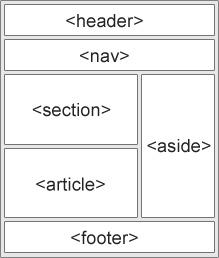
\includegraphics[width=0.7\linewidth]{img_sem_elements}
			\caption{Basic breakdown of semantic html (source: w3schools)}	
		\end{figure}
	
		\begin{description}
			\item[Article:] Makes sense on it's own, the content should be understandable regardless of the rest of the site
			\item[Aside:] Content placed to the side, related to surrounding content
			\item[Details:] Additional details the user can show or hide on demand
			\item[FigCaption:] Caption for an image
			\item[Figure:] Defines an image, typically includes a \texttt{figcaption}
			\item[Footer:] Footer of a document or section. Typically: Author, Copyright Information, Links to Terms of Use, Contact Information, etc
			\item[Header:] Header of a document or section
			\item[Main:] Main content of the document
			\item[Mark:] Highlights part of the text
			\item[Nav:] Block for major navigational links
			\item[Section:] ``A section is a thematic grouping of content, typically with a heading''
			\item[Summary:] Defines a visible heading for the details tag
			\item[Time:] Defines a human readable date/times
		\end{description}
		
		\section{CSS Selectors}
		\begin{description}
			\item[.class] Selects all elements with class equal to ``class''
			\item[\#id] Selects all elements with id equal to ``id''
			\item[*] Selects all elements
			\item[element] Selects all elements by tag name
			\item[element,element] Multiple css selectors
			\item[element element] Selects all elements inside an element
			\item[element > element] Selects all direct children of an element
			\item[element + element] Selects all elements directly after an element
			\item[element ~ element] Selects all elements preceded by an element
			\item[{[attribute]}] Selects elements with the attribute
			\item[{[attribute=value]}] Selects elements with attribute equal to value
			\item[{[attribute~=value]}] Selects elements with attribute containing value
			\item[{[attribute|=value]}] Selects elements with attribute starting with value
			\item[{[attribute\^=value]}]
			\item[{[attribute\$=value]}] Selects elements with attribute ending with value
			\item[{[attribute*=value]}] Selects elements with attribute containing substring value
			\item[:active] Selects the active link
			\item[::after] Insert something after the content
			\item[::before] Insert something before the content
			\item[:checked] Selects every checked input
			\item[:default] Selects the default input
			\item[:disabled] Selects every disabled input
			\item[:empty] Selects parents with no children
			\item[:enabled] Selects every enabled input
			\item[:first-child] Selects if first child of parent
			\item[::first-letter] Selects the first letter
			\item[::first-line] Selects the first line
			\item[:first-of-type] Selects if first element of parent
			\item[:focus] Selects input which has focus
			\item[:hover] Selects if mouse is over
			\item[:in-range] Selects input elements with a value specified within a range
			\item[:indeterminate] Selects input elements that are indeterminate
			\item[:invalid] Selects all input elements with an invalid value
			\item[:lang(language)] Selects with lang attribute equal to language
			\item[:last-child] Selects elements that are the last child of the parent
			\item[:last-of-type] Selects elements that are the last child of the parent
			\item[:link] Selects all unvisited links
			\item[:not(selector)] Selects every element that is not the element
			\item[:nth-child(n)] Selects every element that is the nth child of the parent
			\item[:nth-last-child(n)] Selects every element that is the last nth child of the parent
			\item[:nth-last-of-type(n)] Selects every element that is the last nth child of the parent
			\item[:nth-of-type(n)] Selects every element that is the nth of type from the parent
			\item[:only-of-type] Selects every element that is the only type from parent
			\item[:only-child] Selects every element that is the only child of its parent
			\item[:optional] Selects inputs with no required attributes
			\item[:out-of-range] Selects input elements with a value outside the specified range
			\item[::placeholder] Selects inputs with a placeholder text
			\item[:read-only] Selects inputs with the readonly attribute
			\item[:read-write] Selects inputs without the readonly attribute
			\item[:required] Selects inputs with the required attribute
			\item[:root] Selects the document's root element
			\item[::selection] Selects the portion of an element that is selected by a user
			\item[:target] Selects the current active element (clicked on a URL containing that anchor name)
			\item[:valid] Selects all input elements with a valid value
			\item[:visited] Selects all visited links
		\end{description}
		
		\section{Background}
		\begin{description}
			\item[background-image:] selects the background image to use, accepted value takes the form \texttt{url("image.jpg")}
			\item[background-color:] specifies the background color in hex
			\item[background-position:] positions the image, accepted values: 
			\begin{itemize}
				\item (left | right | center) (top | bottom | center)
				\item x\% y\%
				\item x y 
				\subitem Position in px
			\end{itemize}
			\item[background-repeat:] enables the image to be repeated, possible values:
			\begin{itemize}
				\item repeat
				\item repeat-x
				\item repeat-y
				\item no-repeat
				\item space
				\subitem repeat without clipping and remaining space distributed evenly
				\item round
				\subitem repeat without clipping and centered	
			\end{itemize}
			\item[background-size:] specifies the size of the background images, possible values:
			\begin{itemize}
				\item auto
				\subitem displayed at original size
				\item \textit{height} \textit{width}
				\subitem sets the image height and width in pixels, percentage is also supported
				\item cover
				\subitem resize the image to cover the entire screen (stretches or cuts off the sides if needed)
				\item contain
				\subitem resize to make the entire image visible
			\end{itemize}
		\end{description}
		
	\end{multicols*}
		
	\section{Code Snippets}

	\subsection{Example Page Layout}
	\begin{lstlisting}
<!DOCTYPE html>
<html lang="en">
<head>
	<meta charset="utf-8" />
	<title>Page Title</title>
	<style>
		:root {
			--primary: #482f40;
		}
	</style>
	<link rel="stylesheet" href="styles.css" />
</head>
<body>
	<img src="image.png" alt="Some Image" />

	<script type="text/javascript" src="scripts.js"></script>
</body>	
	\end{lstlisting}
	

	\subsection{Details}
	\begin{lstlisting}[language=html]
<details>
	<summary>World's Tallest Mountain</summary>
	<p>Here you would place some information about the worlds tallest moon</p>
</details>
	\end{lstlisting}
\end{document}
